Tutto quello che accade nell'Universo lo possiamo sapere soltanto analizzando la radiazione elettromagnetica, quindi dobbiamo cercare in essa la firma dei processi che l'hanno prodotta (la radiazione infatti viene emessa in modo diverso a seconda del processo).

La radiazione riflessa, per esempio, è polarizzata e possiamo sfruttare le proprietà della polarizzazione per studiare, per esempio, i processi che accompagnano una stella avvolta da un disco: infatti in tal caso la luce che arriva a noi è in parte riflessa dal disco e quindi polarizzata.

La luce può essere scatterata dalle particelle (es. polvere in aria). Nel caso dei gamma può avvenire il Compton inverso: la radiazione può cambiare la sua frequenza se interagisce con una particella che le cede la sua energia cinetica.

Il Cherenkov\footnote{Emissione di radiazione quando un mezzo è attraversato da una particella carica con velocità maggiore di quella della luce nello stesso mezzo} inverso è invece un processo che accade se e solo se la particella è relativistica: questa particella in genere è prodotta da reazioni nucleari, essa non può essere prodotta in altro modo.

Un altro esempio di emissione dovuta a particelle relativistiche è la radiazione di sincrotrone. Il sincrotrone è un acceleratore che grazie alla presenza di campi magnetici fa si che la traiettoria dell'elettrone sia circolare, ma quando una particella carica viene accelerata (in questo caso è una accelerazione centripeta) irraggia: la radiazione emessa da elettroni in moto su una traiettoria circolare si chiama radiazione di sincrotrone. Questa emissione avviene nel radio e porta la firma dell'elettrone e del campo magnetico che l'ha curvato.

Dall'analisi della radiazione possiamo capire quale evento l'ha generata: per esempio nel Sole si generano particelle cariche a velocità relativistiche che risentono del campo magnetico solare emettendo radiazione di sincrotrone; non vediamo la particella, ma dalla luce di sincrotrone ricostruiamo l'ambiente che l'ha prodotta.

Ovviamente non è detto che il problema abbia un'unica soluzione, nel senso che si potrebbero avere altre condizioni che generano la stessa radiazione: bisogna allora cercare conferma in altri fenomeni. Consideriamo infatti l'urto tra due atomi di idrogeno: durante la collisione viene trasferita energia, l'elettrone passa al livello più alto e poi decade emettendo un fotone di lunghezza d'onda caratteristica del salto energetico nel sistema di riferimento dell'atomo che emette. Se l'atomo si muove la lunghezza d'onda misurata da un osservatore fermo è diversa per effetto Doppler, e la differenza ci da informazioni sulla velocità dell'atomo che emette. In questo modo abbiamo una conferma che si tratta di Cherenkov inverso.
%Se ho una massa di atomi di idrogeno che viene attraversata da un protone a velocità relativistiche; può succedere che uno di questi protoni rubi un elettrone a un atomo e lo colloca a un livello alto, questo decade con una velocità che non è quella ordinaria, ma è molto grande: questa è la conferma che esistono protoni ad altissima energia e quindi il Cherenkov inverso è vero.
Bisogna usare tutto ciò che conosciamo sulla interazione radiazione-materia per estrarre informazioni sulle sorgenti.

\subsection{Acquisizione dati in astrofisica}
Supponiamo di voler studiare oggetti nel cielo analizzando la radiazione: nella pratica significa che a un certo istante di tempo guardiamo in una direzione e riceviamo una intensità specifica (una misura dell'energia normalizzata da tutto ciò che potrebbe alterarla), che cambia con la posizione, con il tempo e con la frequenza.

\E importante conoscere lo strumento con cui sono state effettuate le misure. Immaginiamo di avere un detector bidimensionale fatto di quadratini che si accendono quando vengono colpiti dalla luce ovunque arrivi il fotone: se arriva un cerchio comunque noi vediamo accendere un quadrato. Quindi dagli strumenti dipende ciò che crediamo di aver visto.

Anche la cadenza con cui si fanno le osservazioni ci può dare un risultato sbagliato. Immaginiamo per esempio una persona che tutte le sere a mezzanotte misura la luce di una stella registrando sempre lo stesso numero di fotoni; egli si convince che l'intensità sia costante, poi fa una misura a notte fonda e si accorge che il risultato è diverso: ciò vuol dire che il fenomeno ha una periodicità che è inferiore a un giorno.

L'importante quando si costruiscono gli strumenti è che essi ci permettano di capire quali sono i limiti della misura, non si può pensare di analizzare un dato per verificare una teoria senza sapere come il dato è stato acquisito.

\vspace{0.2cm}Ci chiediamo adesso come si fa a ottenere un'immagine del cielo sapendo che questa dipende dalla lunghezza d'onda. Gli strumenti infatti danno tutti una risposta di tipo si/no (si accendono o non si accendono), essi ci permettono di misurare l'intensità, ma non il colore. Allora come fa la macchina fotografica a fare le foto a colori? Questa è fatta da tanti dispositivi, davanti ai quali ci sono dei filtri colorati rosso, giallo e blu; si fa la conta dei fotoni dei tre colori e in base a ciò si produce la foto a colori, ma non sono esattamente gli stessi colori che vediamo.

Dobbiamo acquisire dati non solo spazialmente, ma anche in lunghezza d'onda. Abbiamo visto che la capacità di risolvere due stelle dipende dal diametro del telescopio in base al criterio di Rayleigh, quindi dobbiamo raccogliere la luce con un grande telescopio, poi questa immagine (disco di Airy) la dobbiamo mettere dentro un sensore. Ricordiamo che una stella di magnitudine $0$ emette $\rm 1000 \; fotoni/(cm^2 \cdot s \cdot \text{Å})$ (questo numero è da ricordare).

\vspace{0.2cm}Il detector lo abbiamo descritto come un oggetto che raccoglie fotoni, ma questo deve avere alcune caratteristiche: idealmente dovrebbe raccogliere fotoni di tutte le lunghezze d'onda (nella realtà non è possibile), inoltre per ogni fotone che arriva deve stabilire l'istante in cui è arrivato e la direzione da cui è arrivato, deve essere in grado di distinguere due fotoni che arrivano quasi contemporaneamente, deve avere un lungo tempo di integrazione (il tempo durante il quale il sensore raccoglie la luce proveniente dalla sorgente) e un numero grande di pixel (per distinguere esattamente la direzione dei fotoni), inoltre lo strumento deve essere in grado di misurare il grado di polarizzazione\footnote{Il grado di polarizzazione di un fotone è una misura della polarizzazione della luce a cui quel fotone appartiene. La polarizzazione si riferisce all'orientamento delle oscillazioni del campo elettromagnetico associato alla luce. In altre parole, indica in quale direzione vibra il campo elettrico della luce.} perché questo ci dà informazioni sulla sorgente. Nella realtà non esiste un tale detector ideale, anche se esistesse avremmo comunque un problema di archiviazione dei dati.

Spesso inoltre gli eventi non sono correlati in maniera lineare (non è che se arrivano due fotoni c'è il doppio di corrente) perché a un certo punto c'è una saturazione: l'aumento eccessivo di luce non produce un ulteriore aumento del segnale.

Ci sono tanti parametri che caratterizzano un detector, i più importanti sono due:

\begin{enumerate}
   \item la \textbf{sensibilità}, o quantum efficiency, che è il rapporto tra il numero di fotoni riconosciuti come eventi diviso quelli incidenti (in genere l'efficienza quantica della CCD\footnotemark di un telescopio è dell'ordine del 95\%, quella della fotocamera di un cellulare è del 30\%);
   \begin{figure}[H]
      \centering
      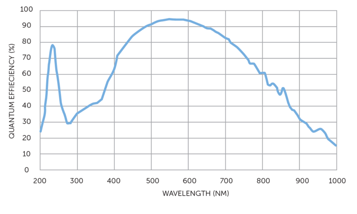
\includegraphics[width=9cm]{astro1.png}
   \end{figure}
   \item il \textbf{range dinamico}, che è la quantità di segnale che può essere registrata: c'è un valore minimo e un massimo, che può dipendere da aspetti hardware o numerici (es. display a 3 cifre).
\end{enumerate}

\footnotetext{Un CCD, o Charge-Coupled Device, è un dispositivo elettronico sensibile alla luce utilizzato in astrofisica e in molte altre applicazioni scientifiche e industriali per la rilevazione e la registrazione delle immagini. Si tratta di un tipo di sensore a semiconduttore che è in grado di convertire la luce in segnali elettrici.}

\vspace{0.3cm}

In passato si usava come detector la lastra fotografica, basata sul fatto che lo ioduro di argento può essere sospeso su una gelatina e quando viene colpito da un fotone produce qualcosa di annerito. La lastra fotografica ha rivoluzionato l'astrofisica perché permette di vedere anche lunghezze d'onda maggiori di quelle che vediamo con i nostri occhi: essa riportava dunque stelle non visibili altrimenti. Il grande svantaggio è che questo strumento è analogico: i dati non possono essere digitalizzati e archiviati.

In seguito sono arrivati i fotomoltiplicatori: all'arrivo di un fotone lo strumento rilascia un elettrone che viene accelerato da una ddp, impatta su una lastra di metallo (dinodo) liberando un numero maggiore di elettroni, che poi vengono accelerati in cascata da una corrente leggibile.

\begin{figure}[H]
   \centering
   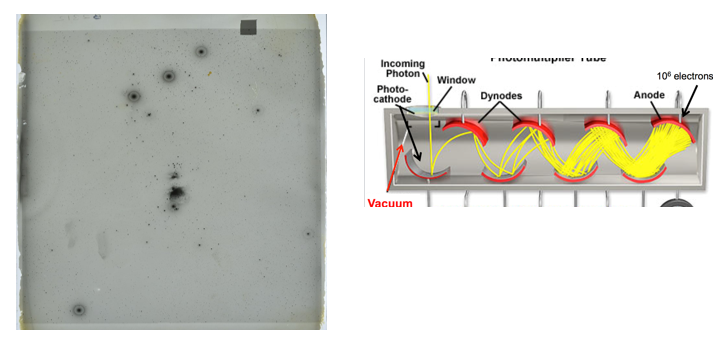
\includegraphics[width=10cm]{astro2.png}
\end{figure}

Oggi si utilizzano i CCD, che sono oggetti tridimensionali, costituiti da una matrice di sensori tutti uguali, con pixel da 4 a 24 micron (quelli usati in astrofisica sono più grandi di quelli presenti nei nostri cellulari). Essi hanno un'altissima efficienza quantica e ricoprono un intervallo di lunghezze d'onda che va dai 300 nm fino al $\rm \mu m$.

I CCD si basano sull'effetto fotoelettrico: arriva un fotone e se ha energia sufficiente libera un elettrone; ovviamente c'è un problema di soglia, nel senso che i fotoni con energia inferiore al lavoro di estrazione non sono rivelabili.

\begin{minipage}{0.4\textwidth}
   \begin{figure}[H]
      \centering
      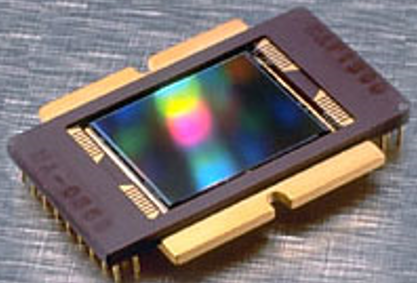
\includegraphics[width=5cm]{astro3.png}
   \end{figure}
\end{minipage}
\begin{minipage}{0.6\textwidth}
   \begin{figure}[H]
      \centering
      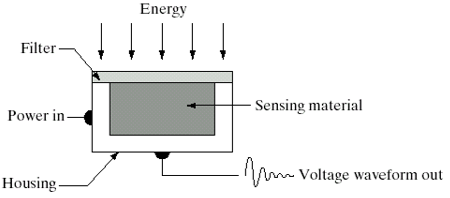
\includegraphics[width=9cm]{astro4.png}
   \end{figure}
\end{minipage}

\vspace{0.3cm}Quando arriva il fotone, un elettrone passa dalla banda di valenza a quella di conduzione; si collocano sopra 3 elettrodi, quello al centro è positivo e i due lateralmente negativi, quindi l'elettrone resta intrappolato. Più fotoni arrivano più elettroni vengono intrappolati, alla fine gli elettroni vengono spostati verso un lettore di corrente cambiando la polarità degli elettrodi (da $-+-$ a $-++$). C'è chiaramente un tempo di lettura non trascurabile.

\begin{figure}[H]
   \centering
   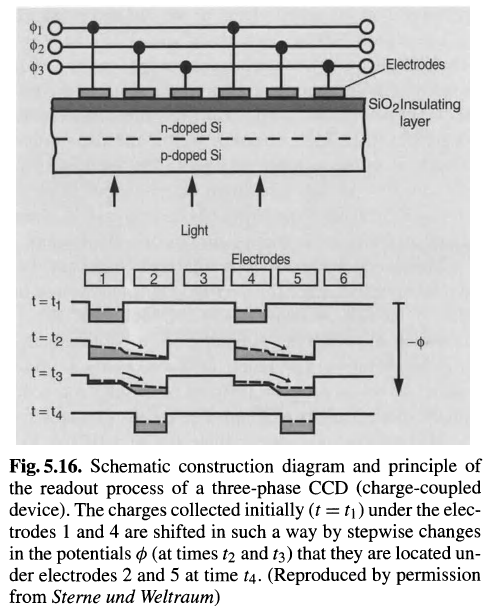
\includegraphics[width=8cm]{immagini/ccd.png}
\end{figure}

Il CCD ha il grande vantaggio di avere una immagine digitalizzata e di darci informazioni sulle coordinate grazie ai pixels. Abbiamo detto che la risposta di una lastra fotografica non è lineare: questa si attiva solo quando è colpita da un certo numero di fotoni, poi la risposta cresce, ma va a saturazione. I CCD invece hanno una risposta lineare. Questi strumenti hanno permesso di migliorare l'efficienza dei telescopi: un telescopio equipaggiato con un CCD può essere più piccolo di un fattore 100 di un telescopio con lastra fotografica e l'efficienza sarà la stessa (ma la risoluzione peggiora).

\begin{figure}[H]
   \centering
   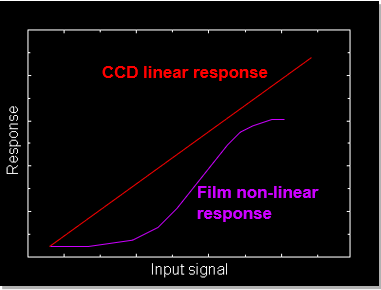
\includegraphics[width=9cm]{astro5.png}
\end{figure}

\subsection{Imaging}
I CCD sono stati inventati negli anni '60 come storage dei computer, ma poi si è capito che si potevano usare come dispositivi fotografici. Vediamo come si fa a trasformare una informazione continua in una immagine pixelata: sappiamo che ogni segnale si può esprimere mediante trasformata di Fourier, ma nella rappresentazione in armoniche c'è un taglio in frequenza sopra e sotto: non potremo mai registrare una lunghezza d'onda maggiore della dimensione del sensore, ma anche le lunghezze d'onda tanto piccole da ricadere tutte all'interno di un pixel si perdono.
 
\begin{figure}[H]
   \centering
   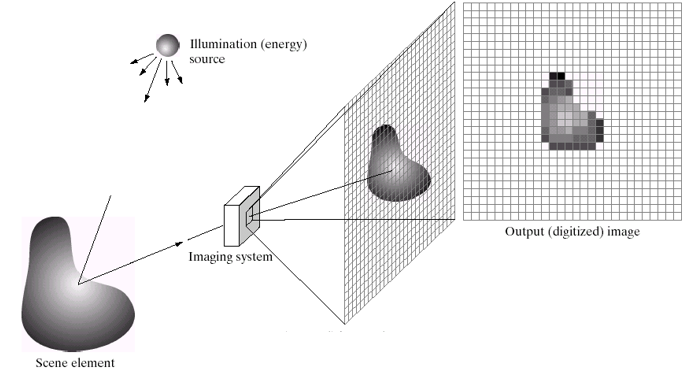
\includegraphics[width=9cm]{astro6.png}
\end{figure}

L'immagine ci appare quindi diversa da come è nella realtà proprio perché si perdono alcune frequenze. Inoltre quando i fotoni presenti in un pixel vengono letti come corrente facciamo una scelta: con quanti bit rappresentare il segnale. Ciò è importante perché il CCD non può contenere troppi elettroni oppure ci può essere una perdita nel processo di archiviazione: alcune informazioni si conservano nell'archiviazione e altre si perdono e ciò determina la risoluzione dell'immagine, ma più informazioni archiviamo più tempo ci vuole. Un'altra grossa limitazione è il numero di pixel: più ne abbiamo, più spazio occupiamo, più tempo serve per trasferire i dati. In base a cosa vogliamo vedere scegliamo le caratteristiche ottimali del CCD.

Inoltre il funzionamento è influenzato dalla temperatura: se si raffredda il CCD allora il numero di elettroni che passano spontaneamente in banda di conduzione è trascurabile, quindi si riducono i rumori. Un vantaggio importante dei CCD è che sono riutilizzabili; inoltre essi sono piccoli, ma si possono mettere più unità in un mosaico.

\subsection{Tecniche astronomiche: fotometria}

Vediamo adesso cosa possiamo dedurre, dal punto di vista quantitativo, misurando la quantità di energia che arriva da una stella.

Abbiamo definito la magnitudine come $-2.5 \log_{10} (F/F_0)$. In questa definizione, la differenza di magnitudine tra due stelle è implicitamente pari al rapporto dei flussi, quindi dà la possibilità di comparare una stella rispetto ad un'altra in termini di percentuali. %In questa scala viene definita come una differenza 

La fotometria nasce come magnitudine visuale (ciò che possiamo vedere) ed in quest'epoca si potevano classificare gli oggetti più brillanti ed evidenziarne lo spostamento nel cielo, quindi abbiamo visto una sorta di astronomia di posizione. La fotometria (come la intendiamo oggi) nasce a metà dell'Ottocento, quando Bond ebbe l'idea di mettere al fuoco del telescopio una macchina fotografica: in questo momento comincia l'utilizzo della fotometria in termini quantitativi. La prima e grande scoperta di Bond nel fare fotografia fu che la dimensione dell'immagine di una stella su un piano focale (lastra fotografica a quell'epoca, oggi CCD) è tanto più grande quanto maggiore è la luminosità dell'oggetto. Si passa quindi da una misura soggettiva sulla brillantezza ad una misura oggettiva, dove misuriamo il diametro dell'immagine della stella. Questo è stato il punto nodale di tutto: si potevano fare delle misure veritiere per tutti ed erano ripetibili, secondo i principi della fisica.

L'ulteriore scoperta di Bond fu che quando osservava la lastra impressionata dalle stelle osservava stelle sulla lastra che non riusciva a vedere ad occhio nudo. Questo pose un grande problema: come era possibile che il cielo sulla lastra fotografica fosse diverso da quello che vediamo con gli occhi? Abbiamo spiegato tale fatto nei paragrafi precedenti: Bond vedeva sulla lastra fotografica oggetti che non vedeva con gli occhi, in quanto la lastra fotografica ha un'efficienza quantica, non tanto più alta, ma quanto molto più estesa in lunghezza d'onda rispetto alla porzione del visibile dell'occhio umano; quindi, la lastra fotografica registra ad esempio fotoni da 300 nm che l'occhio umano non vede. A questo punto si definisce una \textit{magnitudine fotografica}, ossia una luminosità degli oggetti diversa dalla magnitudine visuale. Il motivo di tale differenza sta nella differenza che la lastra fotografica riesce a registrare tutta la lunghezza d'onda, poiché effettivamente non tutti gli oggetti emettono allo stesso modo: ci sono oggetti che emettono più a lunghezze d'onda lunghe (ultravioletto) e altri oggetti che emettono di più a lunghezze d'onda più brevi (infrarosso).

In conclusione, vedere in maniera diversa in realtà significa vedere corpi con proprietà emissive diverse. Se quindi riusciamo ad associare un flusso alle lunghezze d'onda, che cosa possiamo misurare? Per dirlo ricordiamo alcuni concetti noti.

\subsubsection{Conoscenze note}
La radiazione apparentemente bianca in realtà è una sovrapposizione spaziale di radiazione di diversa lunghezza d'onda, che si possono separare con uno strumento chiamato spettrografo e che può essere rappresentato con un triangolo di vetro; il motivo per cui si separano è che l'indice di rifrazione dipende dalla lunghezza d'onda, per cui i fasci si piegano in modo diverso e in conseguenza a ciò vedremo la stella scomposta nei suoi diversi colori.

Questo primo esperimento fu condotto da Fraunhofer agli inizi del 1800 con la luce del Sole; egli ottenne lo spettro\footnote{Lo spettro di una sorgente luminosa è la distribuzione della quantità di energia in funzione delle diverse lunghezze d'onda. Può essere continuo o discreto.} del Sole e si accorse che aveva una diversa luminosità con i colori, ma in più si rese conto che lo spettro era attraversato da bande in assorbimento, cioè da strisce buie, che Fraunhofer catalogò con delle lettere dell'alfabeto.

Che cosa stesse vedendo fu un mistero per più di 50 anni, quando finalmente due chimici tedeschi, Kirchhoff e Bunsen, in laboratorio fecero spettri di fiamme: avevano un fornelletto in cui bruciavano i sali. Si accorsero che lo spettro di queste fiamme era sostanzialmente nero con la lunghezza d'onda, ma solcato da righe luminose che cadevano in regioni diverse e quindi si vedevano con colori diversi. L'esperimento successivo che si sono inventati è stato quello di interporre al becco di Bunsen che bruciava sostanze una sorgente continua e scoprirono che la sorgente continua, a differenza di quello che si aspettavano, non dava origine ad un arcobaleno, ma questa volta quelle che prime erano emissioni di luce qui apparivano come bande nere e quindi era un assorbimento: mancava la luce laddove invece qui risultava presente. Questi esperimenti sono stati di fatto la nascita dell'astrofisica, cioè l'idea di poter applicare le leggi della fisica per la convenzione degli astri. 

\subsection{Applicazione nello spettro solare}
Nel Sole abbiamo a che fare con una distribuzione continua della luce e delle bande in assorbimento. Cerchiamo di associare a queste due proprietà un'origine.

Nell' '800 ci si rese conto che la distribuzione dello spettro, quindi la distribuzione dei fotoni con la lunghezza d'onda dei corpi, cambiava con la lunghezza d'onda. Kirchhoff registrò lo spettro di corpi con temperature diversa; il risultato fu che un corpo caldo produceva uno spettro con una forma caratteristica, il quale presentava un massimo che andava sempre a lunghezze d'onda più brevi man mano che la temperatura del corpo aumentava.

Questo andamento caratteristico è descritto matematicamente dalla \textbf{Planckiana}. La distribuzione di Planck dice che tutto dipende da un'unico parametro: la temperatura, tutto il resto sono costanti: velocità della luce, costante di Planck, costante di Boltzmann (che si utilizza per convertire i gradi in energia). Quest'andamento non è tipico dei corpi caldi, intesi come oggetti che possiamo mettere su una fiamma e far bruciare, è in realtà tipico dei corpi neri, in cui si raggiunge una condizione di equilibrio tra la temperatura e la radiazione: Questa condizione è difficile da riprodurre, ma si può riprodurre in maniera ragionevole in laboratorio contenendo la materia all'interno di una sfera, di modo che la radiazione vada in equilibrio con la sfera stessa; se poi pratichiamo un piccolo foro, possiamo vedere questo tipo di emissione.

Questo esperimento fu condotto da Kirchhoff nel 1860, il quale aveva una “lavatrice”, guardava dall'oblò e riscaldava. Sebbene i limiti tecnologici gli impedivano di raggiungere le temperature necessarie, egli intuì questo andamento. %(come la scrivo? pensavo tipo riuscì comunque ad osservare questo andamento).

Grazie al fatto che la distribuzione sia una planckiana per un corpo nero, nasce la possibilità di associare la posizione del massimo alla temperatura: 

\begin{figure}[H]
   \centering
   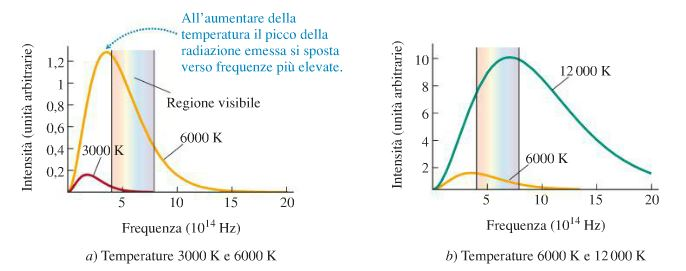
\includegraphics[width=12cm]{immagini/legge_di_wien.png}
\end{figure}

nel grafico vediamo come il massimo di un corpo nero con temperatura 6000 K cada esattamente tra il verde e il giallo, dove cade lo spettro del Sole. Allora è possibile dire che la superficie del Sole ha temperatura di 6000 K.

Dalla distribuzione continua di un corpo possiamo estrarre la temperatura grazie la Legge di Wien:

$$\lambda_{max}=\frac{b}{T}$$

Inoltre, se si fa l'integrale di questa planckiana si ottiene una quantità che cresce con la quarta potenza della temperatura (legge di Stefan-Boltzmann). Questa trattazione però è valida a terra, noi che cerchiamo di associare un concetto di temperatura agli astri non possiamo partire dal principio che la stella sia una planckiana, perché non lo sappiamo ancora. Quello che sappiamo è che il Sole, come tutte le stelle, ha una distribuzione di spettro continuo e l'area sottesa prende il nome di \textbf{magnitudine bolometrica}. In altre parole, facendo l'integrale dello spettro otteniamo l'energia totale, e ipotizzando che il Sole sia assimilabile ad un corpo nero possiamo associare ad esso una temperatura semplicemente dividendo per la costante di Stefan-Boltzmann.

Fare una misura totale del Sole non è impossibile, per esempio nel visibile bastano una lente ed un bicchiere d'acqua con un termometro dentro e all'aumento di temperatura nel termometro si associa una quantità di energia, che è proprio quella che il Sole vi proietta.

Quindi in linea di principio, se abbiamo una distribuzione di spettro, anche se non è effettivamente una planckiana possiamo associare un concetto di temperatura, ma considerando che il Sole è un oggetto esteso e che ogni elemento infinitesimo si comporta come un corpo nero, si definisce la \textbf{temperatura efficace} di una stella come la temperatura tale che la luminosità misurata sia pari a $L=4\pi r^2 \sigma_B T^4$, con $r$ raggio della stella e $\sigma_B$ la costante di Stefan-Boltzmann. %Questa è tale da estrapolare l'energia dal volume emittente, \textbf{nel senso che è per unità di volume?}
In altre parole, la temperatura efficace è la temperatura equivalente di un corpo nero ideale che ha la stessa luminosità della stella.

A questo punto possiamo attribuire alle stelle un valore di temperatura sulla base di questa distribuzione e pensare che la distribuzione continua che osserviamo provenire dal Sole sia dovuta ad un equilibrio tra radiazione e materia.

\vspace{0.2cm}N.d.r.: Secondo me non è ben specificato ma le stelle, essendo assimilate a corpi neri, devono emettere a tutte le frequenze. Nella realtà poi, in base alla composizione e alla temperatura, lo spettro si discosta da quello ideale. 

\vspace{0.2cm}Rimane da capire cosa fossero le bande di assorbimento che solcavano lo spettro dal Sole osservato da Fraunhofer. Per questo richiamiamo i concetti riguardo l'atomo di idrogeno ed i suoi orbitali.

Nella figura si mostra come l'atomo di H, che è l'atomo più comune in quanto elemento primario dell'Universo (è presente al 90\% in particelle e al 75\% in massa, quindi è di fatto quello che emette di più). L'atomo di idrogeno è rappresentato con una carica positiva al centro e con le orbite degli elettroni attorno; gli elettroni occupano stati di energia quantizzati: non tutte le orbite sono possibili, perché l'energia e il momento angolare è quantizzato (se così non fosse l'elettrone compierebbe un moto a spirale intorno al nucleo percorrendo orbite sempre più piccole, ed essendo una particella carica emetterebbe radiazione di sincrotrone con conseguente perdita di energia e collassando quindi sul nucleo, come avviene con un satellite artificiale che incontra l'atmosfera nella Terra (infatti i satelliti vanno rispediti in alto perché con l'attrito dell'atmosfera perdono energia e quindi tendono a cadere)).

Per passare da un'orbita all'altra ci vuole un'energia ben precisa. Dalla meccanica quantistica sappiamo che un fotone di frequenza $\nu$ possiede un'energia $h\nu$, e con uno spettro continuo come quello di corpo nero in cui sono presenti tutte le frequenze, quando questa radiazione incontra un atomo di idrogeno ci sarà sicuramente, tra tutte, una frequenza tale da produrre un salto da un livello energetico ad un altro perché $h \nu$ coinciderà esattamente con la differenza di energia di questi livelli. 

\begin{minipage}{0.5\textwidth}
   \begin{figure}[H]
      \centering
      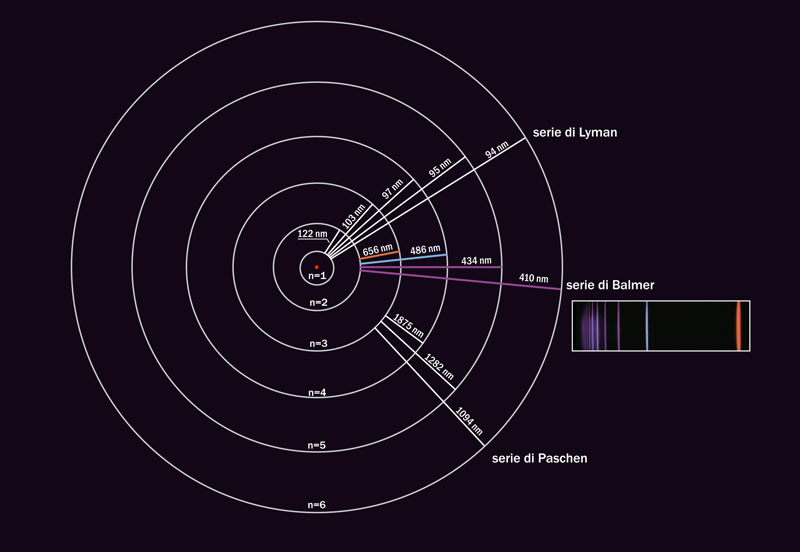
\includegraphics[width=8cm]{immagini/serie_balmer_1.png}
   \end{figure}
\end{minipage}
\begin{minipage}{0.5\textwidth}
   \begin{figure}[H]
      \centering
      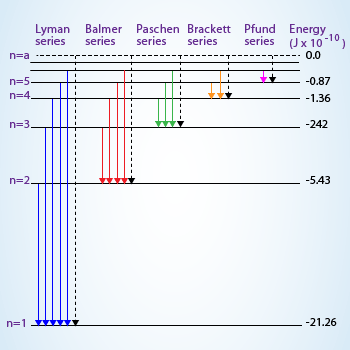
\includegraphics[width=6cm]{immagini/serie_balmer_2.png}
   \end{figure}
\end{minipage}

\vspace{0.3cm}Quali sono queste transizioni? Nel caso dell'atomo di idrogeno le prime scoperte furono quelle del visibile, che sono quelle che coinvolgono il livello energetico $n=2$, per cui per passare dal livello 2 al livello 3 è necessario un fotone di lunghezza d'onda 656 nm o 6563 \AA; questa è una riga fondamentale in astrofisica perché è la più utilizzata visto che sta nella regione del visibile. Poi ci sta la 2 a 4 va a 486 nm e così via. Si definisce serie l'insieme di tutte tutte le transizioni che partono dallo stesso livello; in particolare la serie che parte dal livello 2 si chiama \textit{serie di Balmer}. All'interno di una serie, le righe vengono classificate con le lettere dell'alfabeto, per cui la prima transizione da 2 a 3 viene chiamata alpha, poi da 2 a 4 beta, da 2 a 5 gamma ecc.
Nel caso dell'idrogeno queste transizioni vengono chiamate $H_\alpha$, $H_\beta$, $H_\gamma$, $H_\delta$.

Storicamente le cose sono andato inversamente: Balmer vide le righe spettrali e, chiedendosi a cosa fossero dovute, giunse alla conclusione che erano dovute a transizioni tra livelli energetici dati; egli osservò che le lunghezze d'onda emesse dall'idrogeno sono legate dalla relazione

$$\frac{1}{\lambda}=R \left( \frac{1}{m^2} - \frac{1}{n^2} \right)$$

inoltre legò la frequenza (e quindi l'energia) con i livelli tramite la formula

$$\nu=\frac{E_0}{h} \left( \frac{1}{m^2} - \frac{1}{n^2} \right)$$

dove i termini tra parentesi vengono chiamati \textit{termini} e indicati con $T_m$ e $T_n$\footnote{Lo so che è ridondante ma è la notazione del prof.}. In particolare per la serie di Balmer si ha

$$\nu=\frac{E_0}{h} \left( \frac{1}{4} - \frac{1}{n^2} \right)$$

Sulla base di tali relazioni, a partire dalle righe spettrali si possono determinare le temperature di un corpo e capire quali sono gli elementi chimici presenti. 

Vediamo adesso come sono fatti gli spettri delle stelle:

\begin{figure}[H]
   \centering
   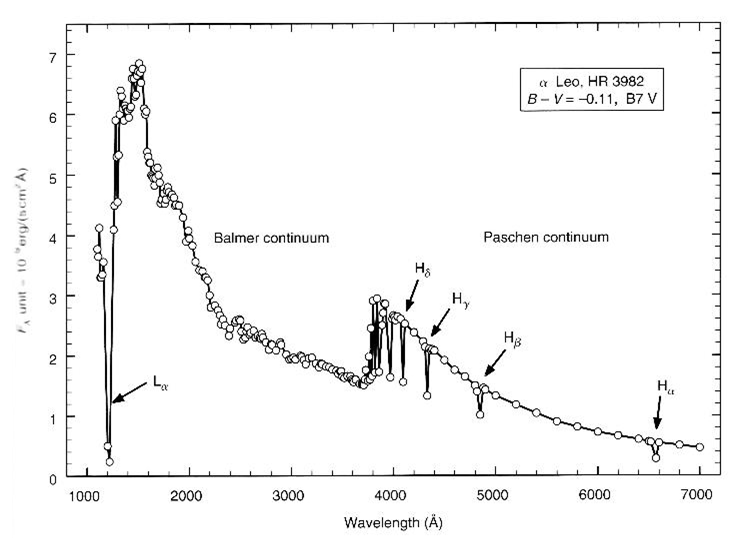
\includegraphics[width=10cm]{immagini/esempio_spettro_stella.png}
\end{figure}

In questo esempio di spettro, compreso tra 1000 e 7000 Angstrom, si ha un comportamento simile a quello a campana che ricorda molto quello di un corpo nero, ma con delle bande in assorbimento; in lunghezze d'onda queste coincidono con le transizioni $H_\alpha$, $H_\beta$, $H_\delta$ e si ha pure la transizione $L_\alpha$, dal livello 1 al livello 2.

Questo andamento non è però del tutto a campana: se guardiamo attentamente il grafico, notiamo che ci sono la transizione da 2 a 3, da 2 a 4, da 2 a 5 ecc.\,, ma effettivamente quanti sono i livelli di un atomo? L'equazione di S. ci fornisce soluzioni per un singolo atomo, per cui si possono avere elettroni a qualsiasi distanza; nel momento in cui abbiamo due atomi, la distanza massima a cui l'elettrone può stare più lontano dal nucleo è pari a metà della distanza tra i due atomi. Quindi quando prendiamo un vero gas o plasma di idrogeno non esistono tutti gli orbitali: avremo un certo numero di orbitali possibili, ma poi l'elettrone passerebbe ad un altro atomo, ed è quello che accade quando la radiazione di cui stiamo discutendo, che ha frequenze sempre più grandi, fornisce quell'energia necessaria per occupare un livello che in realtà non esiste: avviene la ionizzazione. Tale effetto è un effetto a soglia, come l'effetto fotoelettrico, nel senso che tutti i fotoni con frequenza ed energia maggiore di una soglia\footnote{Si parla di energia di Fermi, che è l'energia di soglia oltre al quale si ionizza l'atomo.} possono ionizzare. Infatti il buco del grafico (Balmer continuum) è la zona del corpo nero che corrisponde a quei fotoni che sono assorbiti per ionizzare.

Allora non siamo molto distanti dal poter dire qual è la temperatura di una stella conoscendo la forma del suo spettro (a patto di apportare alcune correzioni):

\begin{figure}[H]
   \centering
   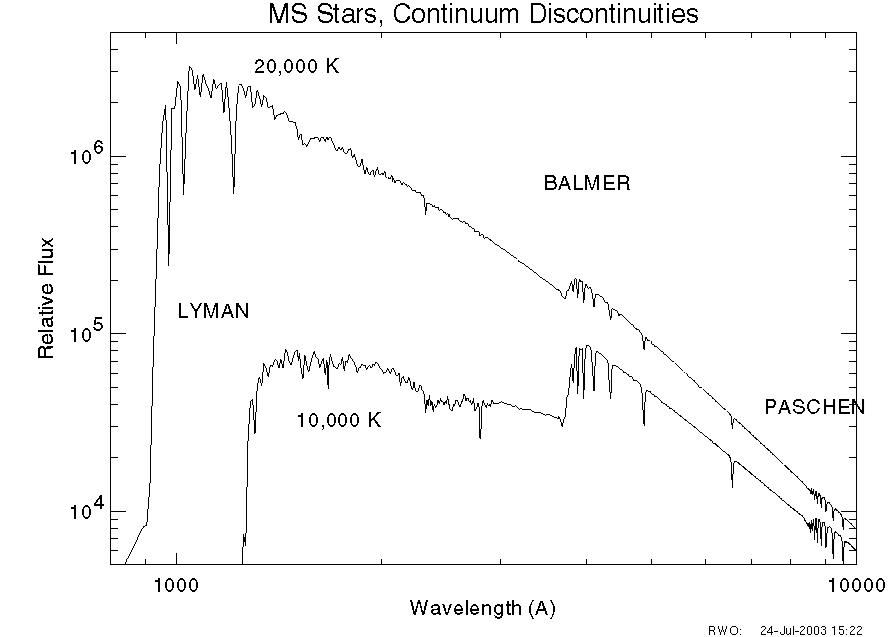
\includegraphics[width=10cm]{immagini/spettro_stella_2.png}
\end{figure}

In figura abbiamo lo spettro di una stella alla temperatura di $1 \cdot 10^3$ K e una alla temperatura di $2 \cdot 10^3$ K. Per la prima il picco corrisponde a quello previsto dalla legge di Wien, mentre per la seconda il picco si sposta indietro e alla $L_{\alpha}$ si sommano quella $\beta$ e $\gamma$, che adesso sono visibili perché nella prima non ci sono fotoni che possono provocare le altre transizioni. In questi spettri distinguiamo un continuo, le righe spettrali, e questi salti che chiamiamo discontinuità di Balmer, che si trova a 3667 \AA.

Se inoltre ordinassimo gli spettri delle stelle in base alla posizione del massimo, scopriremmo che le temperatura vanno da meno di 3000 K fino a 35000 K, e queste sono le temperature che riusciamo ad associare alle stelle.

Questo è l'impianto dal quale partiamo per determinare la temperatura di una stella, cioè la prima applicazione che è stata fatta della misura del flusso è stata quella di associare quella che abbiamo chiamato temperatura efficace. Praticamente come si fa? 
 
\subsubsection{Filtri UBV}

Si può pensare di misurare il flusso all'interno di bande spettrali e determinare, a partire dalla differenza di luminosità della stella all'interno di queste, la temperatura della Planckiana. \E possibile determinare in maniera univoca la temperatura misurando la luminosità soltanto in due bande.

Agli inizi del '900, Johnson inventò un sistema fotometrico basato prima sui 3 filtri U, B, V: essi corrispondono rispettivamente a Ultravioletto (che si colloca prima della discontinuità di Balmer), Blu (che si colloca dopo la discontinuità di Balmer) e Visibile. In seguito furono aggiunti altri due filtri, red ed infrarosso. Questo filtri rappresentano uno standard; li usiamo perché non esiste uno strumento in grado di misurare l'intero spettro, quindi per facilità tecnica ci limitiamo ad un intorno.

Supponiamo di misurare il flusso all'interno di queste bande (per fare ciò è sufficiente far passare la luce attraverso un vetro che trasmette la luce che vogliamo far passare). Quando abbiamo parlato delle magnitudini delle stelle abbiamo detto che essa è data da $ -2.5 \log(F/F_0)$ e, date due stelle, la differenza di magnitudine è pari al rapporto del flusso; adesso applichiamo questo concetto alla stessa stella, utilizzando però due bande diverse: eseguiamo una misura nel filtro B e una misura nel filtro V. La loro differenza coinciderà con il rapporto, e quindi con la pendenza, della planckiana. 

Quando si ha a che fare con misure di questo genere, in cui si calcola la differenza di due magnitudini, si parla di \textbf{indice di colore}, che indica qual è la pendenza del colore e che solitamente si indica con il filtro di lunghezza d'onda più breve del primo:

\begin{equation}
   B-V \equiv m_B -m_V=-2.5 \log_{10} \frac{F_B}{F_V}
\end{equation}

L'applicazione di filtri UBV allo spettro stellare equivale matematicamente a una "media pesata". In altre parole, per ottenere la misura della luminosità di una stella attraverso ciascun filtro UBV, si moltiplica lo spettro stellare per la funzione di trasmissione del filtro (spettro di trasmissione) associato a quel filtro e quindi si integra su tutto lo spettro di trasmissione e lo spettro stellare. Questo processo è noto come "convoluzione spettrale" o "media ponderata spettrale".

Se $S(\lambda)$ rappresenta lo spettro stellare, e $T_U(\lambda), T_B(\lambda)$ e $T_V(\lambda)$ rappresentano le funzioni di trasmissione dei filtri U, B e V rispettivamente (funzioni diverse da zero nella banda e uguali a zero altrove), la misura della luminosità attraverso ciascun filtro è data rispettivamente da:

$$U = \int S(\lambda) \cdot T_U(\lambda) \; d\lambda$$
$$B = \int S(\lambda) \cdot T_B(\lambda) \; d\lambda$$
$$V = \int S(\lambda) \cdot T_V(\lambda) \; d\lambda$$

Queste equazioni rappresentano l'integrazione del prodotto tra lo spettro stellare e la funzione di trasmissione del filtro su tutto lo spettro di lunghezze d'onda ($\lambda$). Il risultato di ciascuna integrazione fornisce la misura della luminosità della stella attraverso il filtro corrispondente (U, B o V).

\vspace{0.2cm}Tuttavia, la luce che arriva sul telescopio è un po' più complicata del flusso della stella, perché la luce della stella deve attraversare l'atmosfera. Bisogna quindi apportare delle correzioni dovute ad esempio alla trasmittanza dell'atmosfera, che può cambiare nel tempo. Misurare la trasmittanza dell'atmosfera terrestre è un processo complesso, che si fa o con dispositivi laser chiamati Lidar, i quali mandano un laser in alta quota e poi ne vedono gli assorbimenti in lunghezza d'onda, oppure dallo spazio. Ma anche la riflettività del telescopio può cambiare nel tempo, ad esempio con l'ossidazione dello strumento. 

Gli astronomi hanno risolto il problema definendo un certo numero di stelle standard, ossia un gruppo di stelle per le quali gli indici di colore sono definiti, cosicché nel momento in cui eseguendo una misura rilevassimo un valore diverso da quello tabulato sapremmo che correzione apportare (ad esempio la stella Vega ha indice di colore $B-V$\footnote{Si legge "B meno V".} uguale a zero, per cui se misurassimo un indice pari a 0.2 sapremmo che dovremmo sottrarre 0.2 a tutte le misure).

Dopo aver apportato queste correzioni è finalmente possibile misurare la temperatura efficace delle stelle semplicemente dall'indice di colore $B-V$. Data la planckiana, si calcola come varia $B-V$ (per farlo è sufficiente fare due foto del cielo con una macchina fotografica in cui una volta montiamo un filtro $B$ e l'altra un filtro $V$) in funzione della temperatura di questa, e il grafico che si ottiene è il seguente:

\begin{figure}[H]
   \centering
   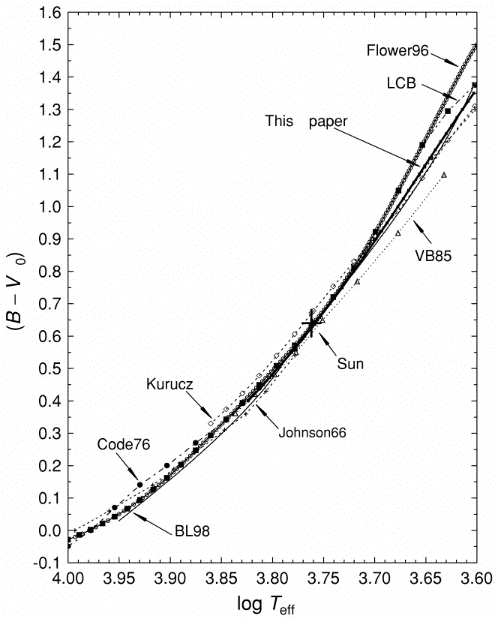
\includegraphics[width=6cm]{immagini/BV_vs_Teff.png}
\end{figure}

\vspace{-0.4cm}

$$\begin{array}{ll}
   B-V=-4.684 \log(T) + 14.551 & \text{per } \log(T) < 3.961\\
   B-V=0.344\big[ \log(T) \big]^2 - 3.402 \log(T) + 8.037 & \text{per } \log(T) > 3.961
\end{array}$$

La temperatura è la prima informazione che si può ricavare da una lastra fotografica, il che è abbastanza intuitivo (nel senso che è intuitivo determinare la temperatura di una stella dal suo colore), ma si può fare molto di più: si può misurare la gravità di una stella, intesa come l'accelerazione di superficie, che dipende dalla sua massa e dal quadrato del suo raggio:

$$g=G\frac{m}{r^2}$$

Bisogna però prestare attenzione ad una cosa: noi siamo in grado di misurare soltanto la massa di stelle appartenenti a sistemi binari, cioè quelle stelle che orbitano a coppia attorno ad un centro di massa comune (il Sole, al contrario, è una stella singola, ma è un caso raro, perché il 70\% circa delle stelle ha un'altra stella come compagna).

Dalla formula di $B-V$ si può ricavare la temperatura efficace $T_{\rm eff}$ e, misurando la quantità di fotoni che arrivano da quella stella, a partire dalla definizione di luminosità $L=4 \pi r^2 \sigma T_{\rm eff}^4$ si può ricavare il raggio della stella.

A questo punto, conoscendo sia il raggio che la massa, è possibile calcolare il valore della gravità superficiale.

\begin{minipage}{0.395\textwidth}
   \begin{figure}[H]
      \centering
      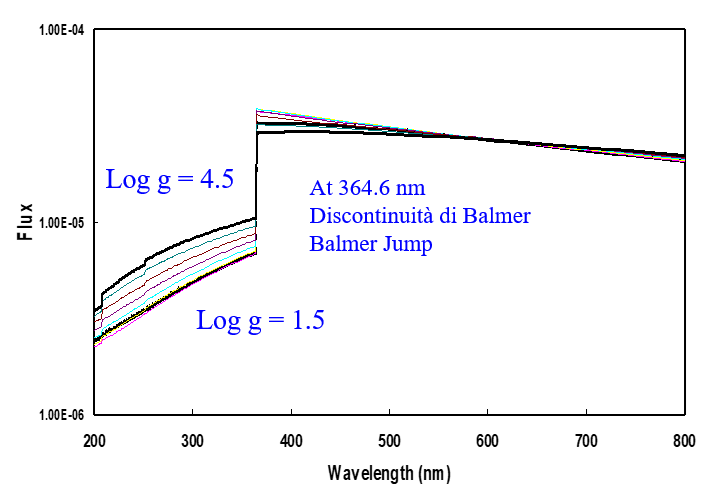
\includegraphics[width=6cm]{immagini/balmer_jump.png}
   \end{figure}
\end{minipage}
\begin{minipage}{0.6\textwidth}
   \vspace{0.4cm}Si è però scoperto che la discontinuità di Balmer (Balmer jump) ha un'ampiezza che, a parità di temperatura, dipende dalla gravità, quindi l'indice di colore $U-B$ può dare una misura dell'accelerazione della stella in superficie e siccome si può fare anche per una stella singola allora si può ottenere la misura della massa di una stella da questo.
\end{minipage}

\subsubsection{Ulteriori parametri ricavabili}

Le stelle non presentano sempre una luminosità costante, e la fotometria è la prima delle tecniche per scoprire fenomeni di variabilità:

\begin{figure}[H]
   \centering
   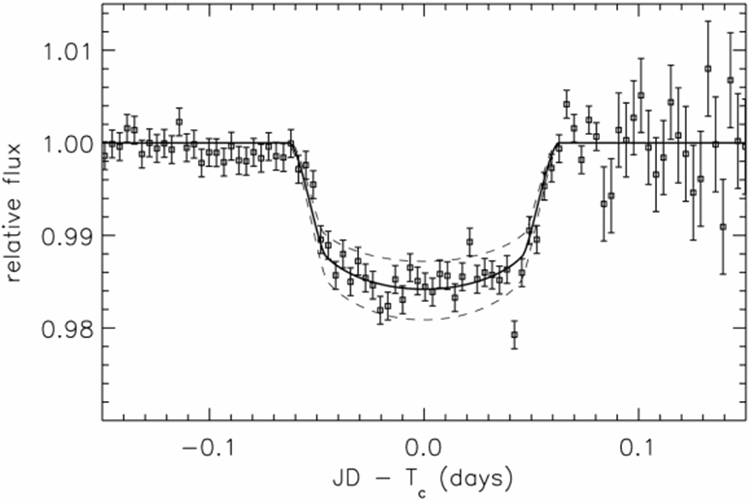
\includegraphics[width=7cm]{immagini/fotometria_luminosita_relativa_1.png}
\end{figure}

\vspace{-0.5cm}

\begin{figure}[H]
   \centering
   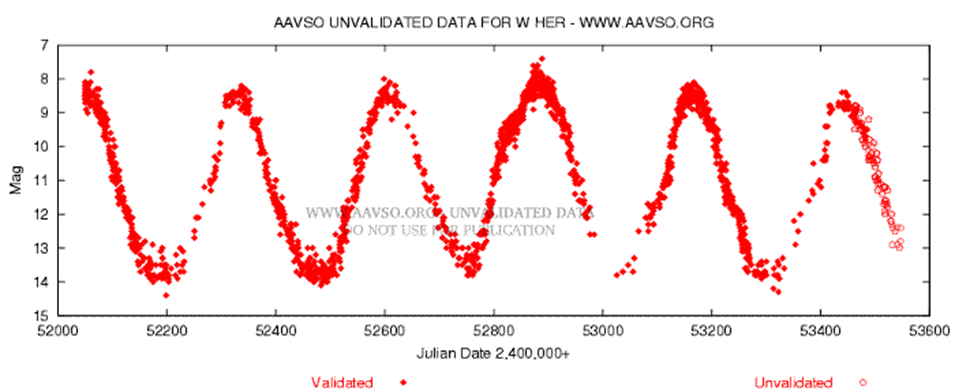
\includegraphics[width=10cm]{immagini/fotometria_luminosita_relativa_2.png}
\end{figure}

In questi grafici sono rappresentate la variazione di magnitudine di una stella per cui si è fatta una misura ogni sera per anni. Quello che si è scoperto è che questa stella cambia la sua luminosità con un periodo di circa 1 anno e varia di ben 6 magnitudini, quindi è una stella che può essere quasi visibile e può scomparire totalmente.

Si può pensare di eseguire queste misure con i filtri $B$ e $V$ in modo tale da calcolare la variazione di temperatura; se poi assimiliamo la stella ad un gas che si comprime ed espande, potremmo ricavare la variazione di raggio della stella.

%Ora lo studio della fotometria permette la scoperta delle variabili fotometriche, però già ci possono essere delle informazioni e quindi se vedo questa mi viene voglia di fare questa misura nel filtro B e V e scoprire quale è la variazione di temperatura e successivamente vista la variazione di temperature, mi viene voglia di capire se questo è semplicemente un gas che si comprime e si espande ed in questo caso potrei ottenere la variazione di raggio della stella.

Dalla variazione luminosa di un corpo (e quindi da un grafico in cui si vede un calo e una risalita) si può raggiungere alla conclusione, ad esempio, che esso venga eclissato dal passaggio di un oggetto. Ne è stato un esempio il passaggio di Venere davanti al Sole. Tale evento conteneva una grande informazione: il raggio del Sole, ricavato a partire dal tempo necessario al transito.

\subsection{Diagramma HR}
La cosa più importante che ha portato la fotometria nell'astrofisica è stata la scoperta fatta da due astronomi indipendentemente, Hertzsprung e Russell, i quali agli inizi del '900, facendo fotometria di tutte le stelle e provando a capire se c'era una relazione tra i parametri come l'indice di colore, le luminosità ecc.\,, costruirono un diagramma, che prende il loro nome, in cui collocarono tutte le stelle, usando come coordinata $x$ l'indice di colore $B-V$ (che come abbiamo visto è una misura della temperatura) ed in $y$ la luminosità:

\begin{figure}[H]
   \centering
   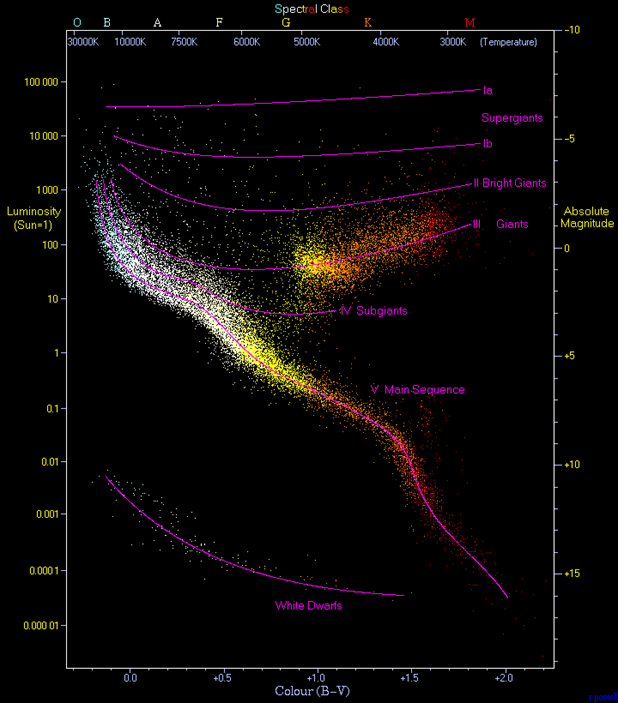
\includegraphics[width=9cm]{immagini/diagramma_HR.png}
\end{figure}

Quello che scoprirono è che il grafico non si riempiva in maniera uniforme, ma vi erano dei luoghi in cui c'era un'alta concentrazione; questi andamenti vennero chiamati \textbf{sequenze}. Quella più affollata fu chiamata \textit{sequenza principale} (da notare che a quell'epoca non si sapeva neanche perché fosse così). Inoltre, in questa distribuzione degli oggetti, i due astronomi si resero conto che a parità di indice di colore e quindi di temperatura, gli oggetti potevano avere luminosità molto diverse. Ricordando che la luminosità è data da $L=4 \pi r^2 \sigma T_{\rm eff}^4$, questa fu intesa come una variazione del raggio della stella, cioè gli oggetti più luminosi erano quelli con il raggio più grande. Per queste motivo le stelle della sequenza principale furono chiamate "nane", mentre le altre subgiganti, giganti e supergiganti, avendo in mente che avessero un raggio molto diverso. Si ha poi un braccio sotto definito come braccio delle nane bianche (la definizione nasce dal fatto che H. e R. potevano vedere solo queste, aventi temperatura 10.000 K, che all'occhio umano appaiono di colore bianco, ma nella teorizzazione moderna del diagramma HR abbiamo un raggio che si estende anche a colori rossi).

Vedendo un grafico come questo, in cui gli oggetti sono organizzati in strutture, ci viene in mente che deve sicuramente esserci una relazione ben precisa tra temperatura, raggio e luminosità; %ma la legge che abbiamo detto finora è soltanto una [1:16:43-45], quindi effettivamente ci vuole una legge che lega 1,2,3 tale che si collochi; quindi noi stiamo collocando in modo ordinato oggetti con una temperatura, un raggio ed una brillanza. Se pensassi al Sole potrei pensare che qui questa legge non esista, perché un oggetto con un certo raggio e una certa temperatura tale da stare qui magari non è in equilibrio stabile; allora è una legge, ma è una legge che magari dice che non sono in condizioni di equilibrio stabile. 

Il diagramma HR può essere immaginato come il periodo più lungo della vita di una stella in cui essa rimane uguale a se stessa.

\textbf{riscrivi}Questo diagramma HR rappresenta il grafico su cui tutti i modelli (intesi come i modelli relativi alle proprietà delle stelle) devono essere valutati. In astrofisica ogni modello deve dare origine a quelle che si chiamano osservabili (se ad esempio facciamo un modello di struttura stellare, bisogna chiedersi quanta luce emette, quanto vale il suo indice di colore, che temperatura e quindi che raggio avrà la stella, ecc.). 

\subsubsection{Ulteriori sistemi fotometrici}

Abbiamo parlato del sistema fotometrico di Johnson come quel sistema fotometrico che campiona lo spettro in alcuni punti. Tale sistema è nato all'inizio del '900, ma in seguito grazie alla tecnologia la nostra conoscenza dello spettro (inizialmente limitata alla regione del visibile, in cui bastano i filtri U, B, V) si è estesa ad altre bande. Per studiarle dobbiamo però estendere i sistemi fotometrici nelle altre bande

\begin{figure}[H]
   \centering
   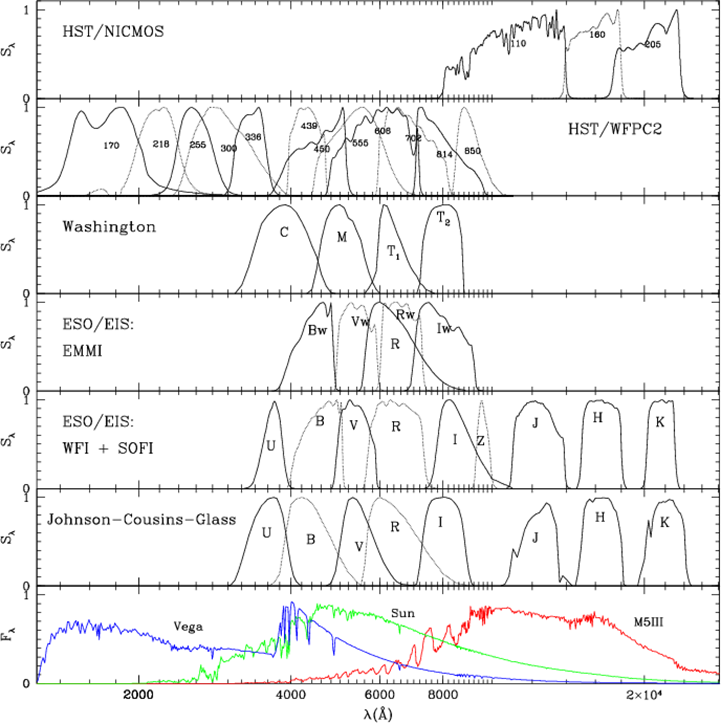
\includegraphics[width=7cm]{immagini/sistemi_fotometrici.png}
\end{figure}

Quello che si è fatto è stato estendere i filtri in altre bande (filtri U.B.V.R.I.J.H.K.), per andare nell'infrarosso e nell'ultravioletto. Tutti questi filtri hanno in generale anche l'obiettivo di riuscire a evidenziare le proprietà di un oggetto, ad esempio individuarne la metallicità.
\begin{figure}[H]
   \centering
   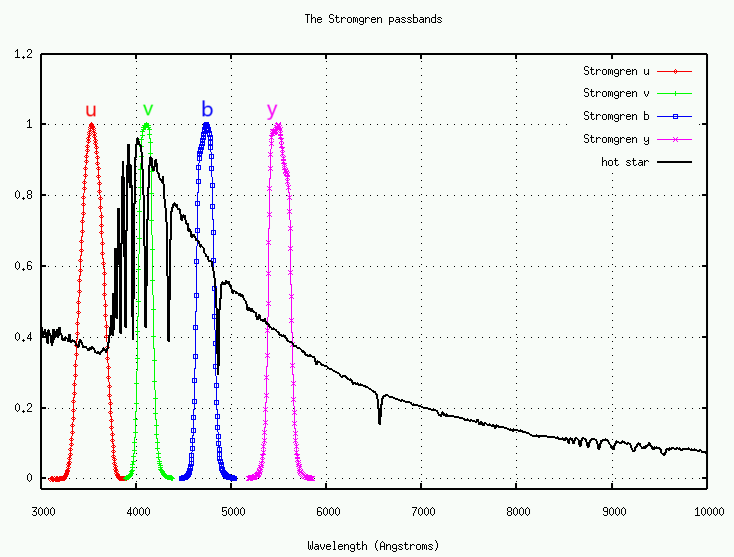
\includegraphics[width=7cm]{immagini/sistema_Stromgren.png}
\end{figure}

Per questa proprietà in particolare si usa il sistema fotometrico Stromgren, che prevede anziché l'uso dei tre filtri di banda larga UBV (1500 Angstrom), quattro filtri di banda stretta (150 Angstrom). Se combiniamo i colori possibili con questi 4 filtri, si riescono a costruire diagrammi (detti diagrammi di colore-colore) tipo quello HR dove le stelle normali occupano ancora una sequenza principale, e gli oggetti peculiari (per esempio per composizione chimica) si presentano fuori.

La realizzazione di diagrammi colore-colore rappresenta ancora una verifica di osservabili. Tra questi ricordiamo il diagramma $m_1$ che mette in evidenza la metallicità e il diagramma c1, che mette in evidenza la gravità.

\subsubsection{Non solo stelle... applicazione alle galassie}

I sistemi fotometrici sono stati pensati guardando le stelle, ma oggi siamo in grado di guardare anche oggetti più lontani delle stelle: le galassie, che sono un'integrale dell'emissività delle stelle, infatti guardando una galassia vediamo la somma di tutte le stelle. Tuttavia, le galassie si allontanano molto rapidamente, dando origine al \textit{redshift}, cioè lo spettro delle galassie appare spostato in lunghezza d'onda per effetto doppler:

$$\frac{\Delta \lambda}{\lambda}=\frac{v}{c}$$

Quindi un oggetto che si muove con velocità $v$ presenta le sue righe spettrali non alla lunghezza d'onda di laboratorio, ma ad una lunghezza d'onda spostata di un $\Delta \lambda$ tale che $\Delta \lambda/\lambda$ sia pari a $v/c$.

\begin{minipage}{0.445\textwidth}
   \begin{figure}[H]
      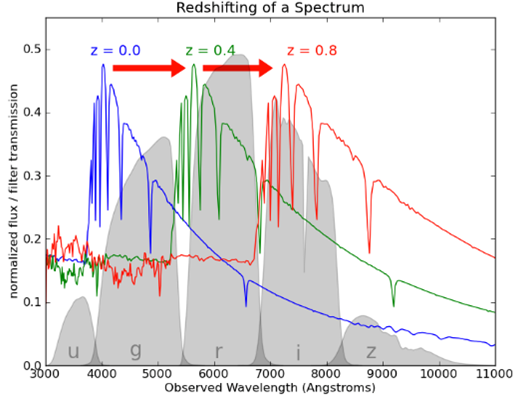
\includegraphics[width=7cm]{immagini/redshift.png}
   \end{figure}
\end{minipage}
\begin{minipage}{0.55\textwidth}
   \vspace{0.4cm}Per tale scopo è stato inventato un sistema fotometrico U.G.R.I.Z.\,, che ha come unico obiettivo la misura dello spostamento della discontinuità di Balmer con la velocità. La velocità in astrofisica è indicata con il parametro $z$ (il motivo è che le velocità sono elevate, per cui non ha senso parlare di km/h) tale che la lunghezza d'onda osservata sia pari ad $1+z$ per la lunghezza d'onda emessa:
   $$\lambda_{\rm obs}=(1+z)\lambda_{\rm emitted}$$
\end{minipage}

\vspace{0.2cm}Allo stato attuale il valore più alto misurato da $z$ è 7.

\subsection{Influenza del mezzo attraversato dalla radiazione}

Le misure di fotometria sono le misure che faremmo se fossimo di fronte ad una stella, ma noi non lo siamo poiché siamo all'interno di un'atmosfera. Cercheremo quindi di capire come si trasforma l'informazione luminosa quando questa interagisce con un mezzo, in particolare con l'atmosfera. Questa infatti non permette il passaggio di tutti i fotoni provenienti dal Sole ad esempio, ma ne fa passare solo una parte.

\begin{figure}[H]
   \centering
   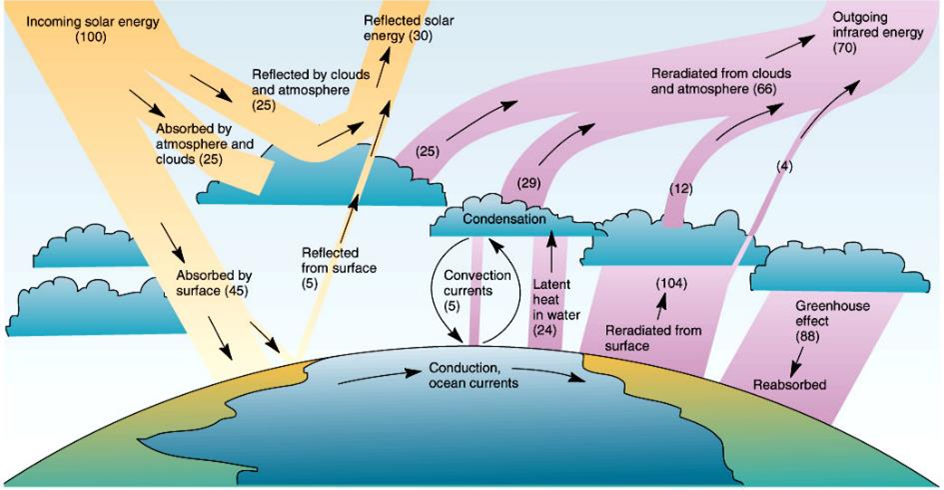
\includegraphics[width=12cm]{immagini/effetto_atmosfera_fotoni.png}
\end{figure}

Ad esempio, su cento fotoni provenienti dal Sole solo cinquanta riescono a raggiungere la superficie terrestre, perché in parte l'atmosfera li assorbe ed in parte li riflette. Per capire come l'atmosfera influenza le nostre misure dobbiamo capire come ogni singolo componente dell'atmosfera (che sappiamo essere composta maggiormente da azoto (78\%) e ossigeno (21\%)) influisce. A proposito di componenti dell'atmosfera riportiamo di seguito un grafico dell'evoluzione nel tempo della quantità di $\rm CO_2$ nell'atmosfera.

\begin{figure}[H]
   \centering
   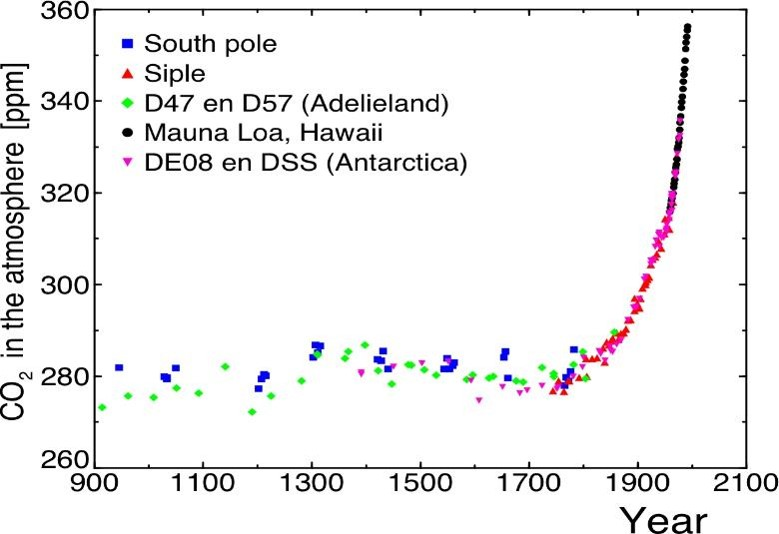
\includegraphics[width=6cm]{grafico CO_2.jpg}
\end{figure}

Come si può notare abbiamo una crescita notevole a partire dalla rivoluzione industriale. I valori dei secoli scorsi sono stati ricavati studiando i ghiacciai. Infatti nel ghiaccio viene conservata la quantità di $\rm CO_2$ presente nell'atmosfera al momento della formazione.

Nell'atmosfera non sono presenti soltanto singoli atomi o molecole ma anche ghiaccio, acqua, particelle e altro che ha dimensioni più grosse di una molecola. Tutti questi componenti sono responsabili dell'assorbimento dei raggi luminosi provenienti dal cosmo.

Cerchiamo di ottenere una rappresentazione più quantitativa di questo fenomeno. Rappresentiamo la quantità di energia che attraversa un piccolo volume di materia con l'intensità specifica\footnote{Ricordiamo che l'abbiamo definita come la quantità di energia che attraversa una superficie normalizzata per l'area della superficie, per la sua proiezione per l'unità di lunghezza d'onda nel tempo, quindi include tutti gli effetti normalizzazione di nostro interesse.} e supponiamo di avere un pennello di energia di radiazione che entra in un cubetto e ne emerge.

\begin{figure}[H]
   \centering
   \begin{tikzpicture}
      \pgfmathsetmacro{\cubex}{1.5}
      \pgfmathsetmacro{\cubey}{1.5}
      \pgfmathsetmacro{\cubez}{1.5}
      \draw[fill=gray!60!] (2.5,0.75,0) -- ++(-\cubex,0,0) -- ++(0,-\cubey,0) -- ++(\cubex,0,0) -- cycle;
      \draw[fill=gray!80!] (2.5,0.75,0) -- ++(0,0,-\cubez) -- ++(0,-\cubey,0) -- ++(0,0,\cubez) -- cycle;
      \draw[fill=gray!50!] (2.5,0.75,0) -- ++(-\cubex,0,0) -- ++(0,0,-\cubez) -- ++(\cubex,0,0) -- cycle;
      \draw[blue!60!cyan!90!, -{Triangle[width = 14pt, length = 8pt]}, line width = 6pt] (2.7, 0.) -- (3.7, 0);
      \draw[blue, -{Triangle[width = 14pt, length = 8pt]}, line width = 6pt] (0.0, 0.0) -- (1, 0.0);
      \node at (-0.3,0) {$I_{\nu}$};
      \node at (4.5,0) {$I_{\nu} - dI_{\nu}$};
      \draw (1,-0.8) -- (1,-0.9) -- (2.5,-0.9) -- (2.5,-0.8);
      \node at (1.75,-1.1) {$dx$};
      \node at (1.75,0) {$\kappa_{\nu}$};
  \end{tikzpicture}
\end{figure}

Siamo sicuri che l'energia uscente dal cubetto sarà minore di quella in ingresso. Vogliamo però quantificare la perdita che si è avuta. Infatti sperimentalmente si vede che la variazione di energia dipende da vari fattori:
    
\begin{itemize}
   \item Dalla quantità di luce che attraversa il nostro volume;
   \item Dallo spessore del nostro volume, in particolare questa dipendenza è lineare (raddoppiando ad esempio lo spessore raddoppiamo la quantità di fotoni persi);
   \item Dal tipo di materiale scelto;
   \item Dalla densità del materiale.
\end{itemize}

La perdita infinitesima di intensità assume dunque la forma:

\begin{equation}
   dI_{\nu}=-k_{\nu} \rho I_{\nu} dx
\end{equation}

dove $dx$ è lo spessore attraversato, $\rho$ è la densità del materiale, $I_{\nu}$ è l'intensità specifica che entra nella superficie considerata, $k_{\nu}$ invece è una costante che dipende dal materiale e dalla frequenza del fotone che attraversa il volumetto infinitesimo. Notiamo che $k_{\nu}$ ha come dimensioni $\rm cm^2/g$, in quanto il prodotto $k_{\nu} \rho dx$ deve essere adimensionale\footnote{La densità in questo caso non è misurata in $\rm kg/m^3$ ma in $\rm g/cm^3$.}. Tale coefficiente è detto \textbf{coefficiente di assorbimento}.

A noi non interessa però esattamente il prodotto $ k_{\nu} \rho \, dx $ bensì il suo integrale lungo tutto lo spessore $L$ del materiale.

\begin{figure}[H]
   \centering
   \begin{tikzpicture}
      \pgfmathsetmacro{\cubex}{4}
      \pgfmathsetmacro{\cubey}{1.5}
      \pgfmathsetmacro{\cubez}{1.5}
      \draw[fill=gray!60!] (2.5,0.75,0) -- ++(-\cubex,0,0) -- ++(0,-\cubey,0) -- ++(\cubex,0,0) -- cycle;
      \draw[fill=gray!80!] (2.5,0.75,0) -- ++(0,0,-\cubez) -- ++(0,-\cubey,0) -- ++(0,0,\cubez) -- cycle;
      \draw[fill=gray!50!] (2.5,0.75,0) -- ++(-\cubex,0,0) -- ++(0,0,-\cubez) -- ++(\cubex,0,0) -- cycle;
      \draw[blue!60!cyan!90!, -{Triangle[width = 14pt, length = 8pt]}, line width = 6pt] (2.7, 0.) -- (3.7, 0);
      \draw[blue, -{Triangle[width = 14pt, length = 8pt]}, line width = 6pt] (-2.5, 0.0) -- (-1.5, 0.0);
      \node at (-2.8,0) {$I_{\nu}$};
      \node at (4.4,0) {$I_{\nu} - dI_{\nu}$};
      \draw (-1.5,-0.8) -- (-1.5,-0.9) -- (2.5,-0.9) -- (2.5,-0.8);
      \node at (0.5,-1.1) {$L$};
      \node at (0.5,0) {$\kappa_{\nu}$};
   \end{tikzpicture}
\end{figure}

Tale integrale è chiamato \textit{profondità ottica} (in inglese optical depth) e viene indicato con $\tau_{\nu}$:

\begin{equation}
   \tau_{\nu} = \int_0^L k_{\nu} \rho \, dx
\end{equation}

Notiamo che a causa della dipendenza della costante di assorbimento dalla frequenza, anche la profondità ottica dipende dalla frequenza del fotone considerato.

Definita questa grandezza possiamo scrivere la variazione infinitesima di intensità come:

\begin{equation}
   dI_{\nu}=- d\tau_{\nu} I_{\nu}
\end{equation}

E risolvendo tale equazione differenziale si ottiene:

\begin{equation}
   I_{\nu}=I^{0}_{\nu} e^{- \tau_{\nu}}
\end{equation}

Quello che capiamo da questa equazione è che la radiazione, attraversando la materia, ha una perdita esponenziale, che può essere calcolata nota l'intensità in ingresso $I^{0}_{\nu}$. Notiamo quindi che il calcolo della perdita di intensità non ha più niente a che fare con la radiazione stessa, bensì si riduce al calcolo di un integrale di quantità che sappiamo misurare.

Analizziamo la dipendenza dalla frequenza facendo un esempio.

%\textbf{STA PARTE E' DA APPROFONDIRE MA NON SO COSA DIRE}

Ci si potrebbe chiedere perché al tramonto il Sole appare rosso mentre a mezzogiorno appare giallo. La risposta sta proprio nei coefficienti di assorbimento relativi alle due lunghezze d'onda. Quando osserviamo il Sole a mezzogiorno, lo strato di atmosfera schermante è di una decina di km, e questo è abbastanza sottile da far passare entrambe le lunghezze d'onda; al tramonto invece le radiazioni dovranno percorrere una spazio decisamente maggiore nell'atmosfera, sufficiente ad assorbire il giallo ma non ad assorbire il rosso. Questo è il motivo per cui non vediamo il sole blu: i fotoni di tale lunghezza d'onda vengono assorbiti dai primi km di atmosfera. In realtà i fotoni non vengono assorbiti nel senso che scompaiono, ma vengono diffusi nel senso che rimbalzano e ritornano indietro, e questo ci fa vedere il cielo blu. Al tramonto invece il colore diffuso è giallo per lo stesso motivo.

Quando parliamo di interazione radiazione-materia possiamo distinguere dei regimi, che sono relazionati dalla dimensione della radiazione rispetto alle dimensioni dell'oggetto responsabile della diffusione. Le tre grandi divisioni si hanno quando la lunghezza d'onda della radiazione ha dimensioni molto più grandi, molto più piccole o comparabili con la dimensione dell'oggetto che stiamo considerando. Un esempio classico quello delle onde del mare che propagandosi incontrano uno scoglio: se lo scoglio è molto piccolo rispetto all'onda, questa passa; se lo scoglio è grandissimo l'onda si interrompe. Quello che è importante notare è la dipendenza dalla lunghezza d'onda, che in generale può essere molto diversa. Se la lunghezza d'onda è comparabile con le dimensioni dell'oggetto, il coefficiente di assorbimento è chiamato più propriamente coefficiente di diffusione, ma ai nostri fini possiamo sempre intenderlo come coefficiente di assorbimento perché i fotoni non arrivano a Terra. Sulla Terra sperimentiamo assorbimenti come $\frac{1}{\lambda}$ e $\frac{1}{\lambda^4}$, oppure si può rilevare il fenomeno dello scattering Thomson\footnote{Tale fenomeno avviene a basse energie (in realtà avviene anche ad alte energie solo che non è visibile perché in quel caso prevalgono altri effetti) e si ha quando sono presenti delle particelle cariche che si muovono a velocità non relativistiche. Quando il fotone "colpisce" la carica questa inizia a oscillare nella stessa direzione del campo elettrico del fotone incidente. La carica in movimento come sappiamo emetterà radiazioni, che avranno la stessa frequenza del fotone incidente ma direzione diversa, in particolare ortogonale al moto della carica.}, che non dipende dalla lunghezza d'onda.

Quindi abbiamo un'ottica geometrica quando la dimensione dell'oggetto è grande rispetto a quella del fotone, in questo caso si hanno fenomeni di scattering, si pensi ad esempio all'ombra che fa un oggetto. Viceversa, se il fotone ha dimensioni molto più grandi dell'oggetto, il primo non si accorge del secondo e passa indisturbato, si pensi ad esempio alle onde radio, anche se mettiamo una persona d'avanti l'antenna riusciamo lo stesso a percepire il segnale.

Come già detto, ognuno dei componenti dell'atmosfera contribuisce all'assorbimento delle radiazioni. Quello più noto è sicuramente l'ozono, che assorbe la radiazioni ultraviolette. In seguito sono riportati dei grafici che mostrano le linee di assorbimento di alcuni componenti dell'atmosfera.

\begin{figure}[H]
   \centering
   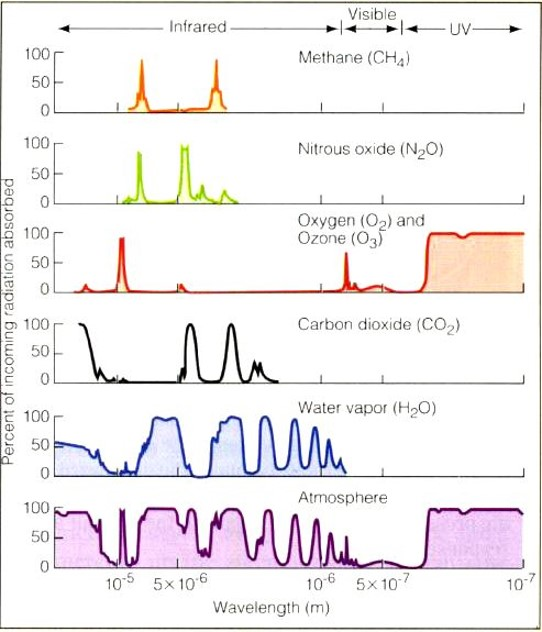
\includegraphics[width=8cm]{righe ass atm.jpg}
   %\caption{Righe di assorbimento di alcuni componenti dell'atmosfera e dell'atmosfera stessa}
   \label{fig:righe_ass_atm}
\end{figure}

Poiché tutte queste componenti convivono nello stesso posto, il risultato che vediamo da terra, chiamato trasmittanza dell'atmosfera, è una somma pesata dei contributi di ognuna di esse avente come peso l'abbondanza di questa nell'atmosfera.

\vspace{0.2cm}Come fanno gli astronomi ad ottenere la misura della magnitudine in un filtro se l'atmosfera la modifica?

\begin{figure}[H]
   \centering
   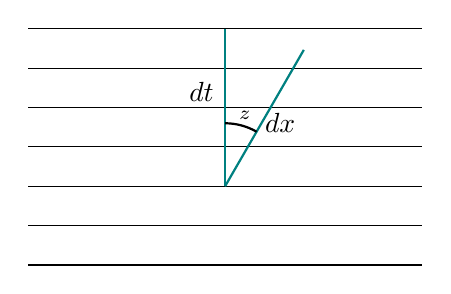
\begin{tikzpicture}
      \foreach \y in {-1.5, -1, -0.5 , 0, 0.5, 1, 1.5}
          \draw[shift={(0,\y)}] (0,0) -- (5,0);
      \draw[thick,teal] (2.5,-0.5) -- (2.5,1.5);
      \node at (2.2,0.7) {$dt$};
      \draw[thick,teal] (2.5,-0.5) -- (3.5,1.232);
      \node at (3.2,0.3) {$dx$};
      \draw[thick] (2.5,0.3) arc (90:60:0.8cm);
      \node at (2.75,0.4) {\scriptsize $z$};
  \end{tikzpicture}
\end{figure}

Consideriamo l'atmosfera terrestre come fatta da tanti strati sovrapposti e supponiamo di avere una stella ad una distanza zenitale $z$ (che ricordiamo essere l'angolo che la stella forma con lo zenith). Indichiamo con $dx$ il cammino percorso dai fotoni, e con $dt$ lo spessore di atmosfera corrispondente al $dx$. I due sono legati dalla relazione:

$$dt=\cos{z} dx \implies dx=\sec{z} dt $$

cioè il $dx$ della profondità ottica si può scomporre come lo spessore $dt$ per la secante di $z$. Quindi il prodotto tra l'intensità fuori dall'atmosfera e l'esponenziale di meno la secante di $z$ per lo spessore ottico è pari all'intensità che misuriamo a terra, cioè:

\begin{equation}
   I_{\nu}=I_{\nu}^* e^{-\sec{z} \tau_{\nu}}
\end{equation}

dove $I_{\nu}^*$ è l'intensità fuori dall'atmosfera.

\begin{minipage}{0.495\textwidth}
   \begin{figure}[H]
      \centering
      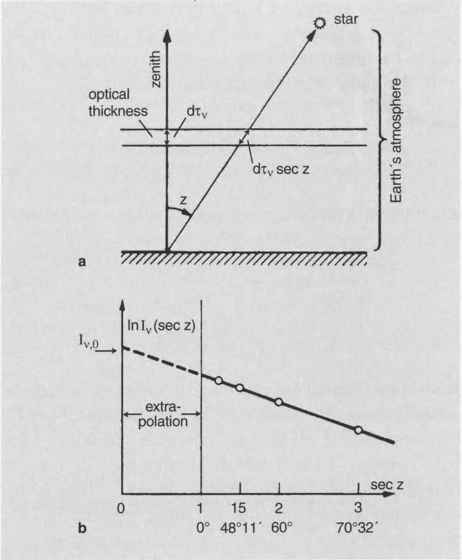
\includegraphics[width=7cm]{immagini/retta_luminosita.png}
   \end{figure}
\end{minipage}
\begin{minipage}{0.495\textwidth}
   \vspace{0.2cm}Gli astronomi non misurano l'intensità ma la magnitudine, che è il logaritmo di questa, e questa relazione in scala logaritmica diventa una retta.
   
   Per trovare quindi la magnitudine fuori dall'atmosfera si eseguono varie misure di una stella ad altezze diverse, partendo da $z$ molto vicini ai 90°\footnotemark fino ad arrivare allo zenith ($z=0$). In questo modo abbiamo dei punti che dovrebbero stare su una retta; tuttavia ancora non abbiamo la misura cercata, perché essa si avrebbe quando $\sec{z}=0$\footnotemark. Ovviamente questa non si può misurare direttamente, ma eseguendo un best-fit con le misure prese possiamo trovare il valore desiderato.
\end{minipage}

\footnotetext{Ovviamente non è possibile farla a 90° a causa degli alberi, dobbiamo metterci a $z$ minori.}

\footnotetext{È evidente che nell'equazione precedente, fissata la stella, la variabile indipendente è $\sec{z}$.}

\subsection{Il mezzo interstellare}

Lo stesso problema che abbiamo con l'atmosfera si avrebbe anche se le misure fossero fatte dallo spazio. Questo perché lo spazio tra le stelle non è vuoto, ed infatti esiste un fenomeno detto assorbimento interstellare, cioè c'è qualcosa (mezzo interstellare) tra le stelle che assorbe le radiazioni. Un esempio si può vedere nella famosa fotografia di una nube scura galattica (Galactic dark clouds) detta testa di cavallo.

\begin{minipage}{0.495\textwidth}
   \begin{figure}[H]
      \centering
      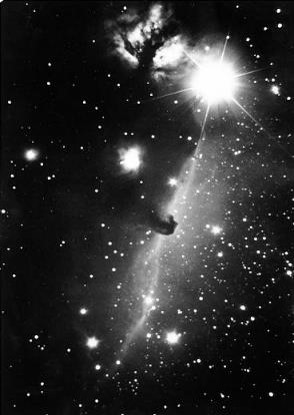
\includegraphics[width=4cm]{horsehead.jpg}
      %\caption{Galactic dark clouds: horsehead}
      \label{fig:horsehead}
  \end{figure}
\end{minipage}
\begin{minipage}{0.5\textwidth}
   \vspace{0.4cm}Nella foto possiamo vedere una stella molto brillante e accanto alla stella c'è una luminescenza, dovuta al fatto che la luce della stella è diffusa da una nube e quest'ultima quindi appare brillante. Possiamo vedere altre zone più scure, che nella foto fanno da contorno a quella che sembra quasi la testa di un cavallo (da qui il nome), che assorbono la luce anziché rifletterla. Quest'ultima nube, proprio perché assorbe, appare nera.
\end{minipage}

\vspace{0.3cm}Vediamo se possiamo applicare in qualche modo quanto detto per l'atmosfera terrestre al caso delle nubi. Il parametro sarà chiaramente diverso: non sarà più l'angolo zenitale, bensì la distanza fisica della nube.

Notiamo alcune differenze. Per le nubi interstellari, a differenza dell'atmosfera, non parleremo più di proprietà ottiche e densità dei vari materiali perché la densità sarebbe troppo bassa (si parla di qualche particella per $\rm km^3$ al massimo), si preferisce piuttosto identificare i vari costituenti in generale con il termine "grani" e considerare la loro densità (misurata in $\rm cm^{-3}$) e non più la loro densità di massa (misurata in $\rm \frac{g}{cm^3}$). Questi grani non devono essere necessariamente atomi, ma possono anche essere corpi dell'ordine di centinaia di micron.

Si avrà quindi che:

$$dI_{\lambda}=-I_{\lambda} \, n(x) k_{\lambda} \; dx$$

dove:

\begin{itemize}
   \item $n(x)$ è il numero di grani per unità di volume, ovvero la densità di grani ($\rm cm^{-3}$);
   \item $k_{\lambda}$ sarebbe il corrispettivo della costante di assorbimento ($\rm cm^2$);
   \item $I_{\lambda}$ è l'intensità del fascio di luce incidente in quello strato.
\end{itemize}

Con gli stessi ragionamenti fatti per l'atmosfera, ma contestualizzati al nostro caso, si ha:

$$I_{\lambda}=I_{\lambda}^0 e^{-\tau_{\lambda}}
\quad\text{con}\quad
\tau_{\lambda}=k_{\lambda} \int_0^x n(x') \; dx'=-k_{\lambda} N(x)$$

dove $I_{\lambda}^0$ è l'intensità intrinseca dalla stella (cioè quella che misureremmo se potessimo andare sulla superficie della stella) e $N(x)$ è la densità di una colonna di grani ($\rm cm^{-2}$), che si può considerare pressoché costante anche se non è esattamente così.

Quello che però alla fine interessa a noi è la magnitudine. Sappiamo che: 

$$A_{\lambda} = -2.5 \log_{10} \left( \frac{I_{\lambda}}{I_{\lambda}^0 } \right)$$

dove $A_{\lambda}$ è una differenza di magnitudine, $I_{\lambda}$ è l'intensità misurata e $I_{\lambda}^0$ è quella intrinseca della stella. Notiamo che il logaritmo utilizzato non è il logaritmo naturale ma quello in base dieci. Nel nostro caso, cioè nel caso in cui la diminuzione di magnitudine sia dovuta ad un mezzo interstellare, la $A_{\lambda}$ viene detta absorption rate. Chiaramente questa dipenderà dalla lunghezza d'onda.

Ricordando che $ I_{\lambda} = I_{\lambda}^0 e^{-\tau_{\lambda}}$ si ottiene:

$$A_{\lambda}=-2.5 \log \left(\frac{I_{\lambda}}{I_{\lambda}^0 } \right)
=-2.5 \log \left( e^{-\tau_{\lambda}} \right)$$
$$=-2.5 \log(e) \ln ( e^{-\tau_{\lambda}} )
=-2.5 (0.4) (-\tau_{\lambda} )
=1.086 \, \tau_{\lambda}$$

Come già detto, questa differenza di magnitudine sembra dipendere dalla lunghezza d'onda, in particolare sembra essere maggiore nella zona degli ultravioletti e minore dell'infrarosso. Questo implica che possiamo guardare sempre più lontano aumentando la lunghezza d'onda, infatti, come detto sopra, all'aumentare della lunghezza d'onda aumenta lo spazio necessario per estinguere quella lunghezza d'onda. Quindi guardando nell'infrarosso o addirittura nel radio possiamo vedere gli oggetti più lontani che altrimenti sarebbero invisibili.

In definitiva l'effetto dell'assorbimento interstellare su un corpo è quello di arrossarlo, cioè lo fa apparire rosso. Dobbiamo però contestualizzare questo concetto di arrossamento in un sistema fotometrico. A questo proposito usiamo il sistema di Johnson UBV (un filtro ultravioletto a 3500 Å, un blu a 4500 Å e un visibile a 5500 Å). Quello che vorremmo fare è ricavare la magnitudine intrinseca da quella osservata. Per farlo però dobbiamo conoscere $A$.

Vediamo come fare. Riprendiamo il concetto di indice di colore: esso è la differenza di magnitudine misurata in due diversi filtri. Fissiamo due filtri $i$ e $j$. Per ognuno di essi avremo una magnitudine osservata e una magnitudine intrinseca, cioè:

$$m_i^{obs} = m_i^{int} + A(\lambda_i) \quad\hbox{ e } \quad m_j^{obs} = m_j^{int} + A(\lambda_j)$$

Indicheremo adesso con $C_{ij}^{obs}$ l'indice di colore osservato, e con $C_{ij}^{int}$ quello intrinseco, cioè:

$$C_{ij}^{obs} = m_i^{obs} - m_j^{obs} \quad\hbox{ e } \quad C_{ij}^{int} = m_i^{int} - m_j^{int}$$

dove il pedice $i$ si riferisce all'indice di colore con lunghezza d'onda più breve tra i due.

Cerchiamo adesso una relazione tra l'indice di colore osservato e quello intrinseco. Notiamo che :

$$C_{ij}^{obs} - C_{ij}^{int} = ( m_i^{obs} - m_j^{obs}) - ( m_i^{int} - m_j^{int} ) = A(\lambda_i) - A(\lambda_j) \equiv E_{ij}$$

dove abbiamo indicato la differenza delle $A$ con $E_{ij}$. Tale parametro è detto \textit{eccesso di colore}. %L'obbiettivo è costruire indici di colori che siano indifferenti all'assorbimento, in modo tale da ottenere informazioni sulla stella anche se la radiazione che produce viene assorbita
%notiamo che abbiamo un eccesso di colore
Quindi per sapere l'indice di colore intrinseco dobbiamo conoscere i valori di $A$ per le diverse lunghezze d'onda. Per trovarci questi valori possiamo pensare di usare delle stelle gemelle al Sole, di cui possiamo pensare di conoscere i parametri intrinseci in quanto li possiamo misurare, come abbiamo già visto, e da quelli ricavare le $A$ come differenza tra le magnitudini misurate per queste stelle e quelle invece intrinseche ottenute dallo studio del Sole. Si è trovato che l'estinzione interstellare ha la forma riportata nel seguente grafico, dove sulle ascisse abbiamo l'inverso della lunghezza d'onda e sulle ordinate l'estinzione:

\begin{figure}[H]
   \centering
   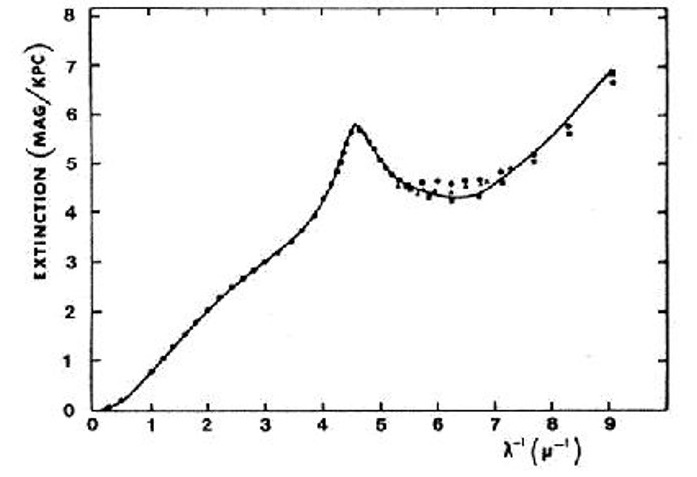
\includegraphics[width=8cm]{estinzione interstellare.jpg}
   %\caption{Andamento dell'estinzione interstellare in funzione dell'inverso della lunghezza d'onda}
   \label{fig:esti inter}
\end{figure}

Notiamo che fino ai 4.5-5 $\rm \mu m^{-1}$ l'andamento è pressoché lineare, molto simile all'estinzione causata dall'atmosfera terrestre, essendo anch'essa causata da molecole. Andando verso le zone dell'ultravioletto invece entrano in gioco anche i grani, che possono essere anche molto più grandi di singole molecole e infatti l'andamento cambia notevolmente. Quindi nella prima parte del grafico, in cui rientra il sistema UBV, possiamo immaginare di costruire un parametro, ovvero il rapporto tra l'eccesso di colore per $U-B$ e quello per $B-V$, che è pari a $1.027$, e da questo possiamo immaginare di determinare la magnitudine intrinseca di un oggetto da quella osservata.

Ci chiediamo adesso qual è la luminosità totale di un oggetto, ovvero l'integrale di tutto lo spettro, dato che noi dello spettro ne prendiamo solo un piccolo pezzetto da Terra, visto che viene in parte assorbito dall'atmosfera e dal mezzo interstellare.

Quello che si è pensato in passato è stato di misurare l'energia proveniente dai corpi vicini (di modo che l'assorbimento interstellare sia piccolo), in maniera indipendente dalla lunghezza d'onda. Per farlo si usano dei particolari dispositivi detti \textit{bolometri}, strumenti capaci di misurare l'energia indipendentemente dalla lunghezza d'onda, che convertono l'energia della radiazione incidente in energia termica, la quale può essere misurata utilizzando un termometro. Posizionando questi dispositivi nello spazio è stato possibile misurare l'energia totale. Questo flusso totale emesso dal corpo è diventato la \textbf{magnitudine bolometrica}, ovvero l'integrale su tutto lo spettro. Questa è una proprietà del corpo, indipendente dalla lunghezza d'onda. Di fatto questo flusso bolometrico altro non è che l'integrale del flusso fatto rispetto a tutte le lunghezze d'onda:

$$F_{Bol} = \int_0^{\infty} F_{\lambda} d\lambda$$

È stata introdotta l'idea di usare un fattore correttivo, chiamata correzione bolometrica, per ricavare dalla magnitudine visuale (quella misurata nella banda del visibile) quella bolometrica.

$$BC= 2.5 \log \left( \frac{F_{bol}}{F_V} \right) + \text{cost.}$$

Inoltre:

$$BC= m_V - m_{bol} = M_V - M_{bol}$$

\textbf{nota che c'è un conflitto di notazione, con le maiuscole si intende quella intrinseca e con le minuscole quella apparente}

Chiaramente questo concetto deve dipendere necessariamente dalla forma dello spettro considerato. Inoltre il fattore correttivo dipenderà anche dalla temperatura della stella: variando la temperatura varia il suo flusso totale. Per questo motivo è stata fatta una campagna osservativa con cui è stata determinata la correzione bolometrica di ogni stella a partire dal suo indice di colore, che è il colore che dà la temperatura.